
%\documentclass[12pt]{amsart}
%\usepackage{geometry} % see geometry.pdf on how to lay out the page. There's lots.
%\geometry{a4paper} % or letter or a5paper or ... etc
% \geometry{landscape} % rotated page geometry

\documentclass[11pt,letter]{article}

%\usepackage[latin1]{inputenc}
\usepackage{epsfig}
\usepackage{amsmath}
%\usepackage{amsfonts}
\usepackage{amssymb}
\usepackage{listings}
\usepackage{booktabs}
\usepackage{setspace}
\usepackage[colorlinks,citecolor=blue]{hyperref}
\usepackage{xcolor}
\usepackage[sort&compress,numbers]{natbib}
%\usepackage{natbibspacing}

\setlength{\oddsidemargin}{.46cm}
\setlength{\evensidemargin}{-0.46cm}
\setlength{\evensidemargin}{0.0cm}
\setlength{\textwidth}{15.5cm}
\setlength{\parskip}{1.0ex plus 0.6ex minus 0.6ex}
\setlength{\parindent}{1.0em} 
\setlength{\textheight}{22.5cm}
\setlength{\topmargin}{-2cm}
\setlength{\footskip}{2cm}
\setlength{\parindent}{0.0cm}

\def\aj{Astron. J.}
\def\apj{Astrophys. J.}
\def\apjl{Astrophys. J. Lett.}
\def\apjs{Astrophys. J. Supp. Ser. }
\def\aa{Astron. Astrophys. }
\def\aap{Astron. Astrophys. }
\def\araa{Ann.\ Rev. Astron. Astroph. }
\def\physrep{Phys. Rep. }
\def\mnras{Mon. Not. Roy. Astron. Soc. }
\def\mmsun{M_\odot}
\def\prl{Phys. Rev. Lett.}
\def\prd{Phys. Rev. D.}
\def\azh{Soviet Astron.}
\def\apss{Astrophys. Space Sci.}
\def\cqg{Class. Quantum Grav.}


\usepackage{mathpazo}
\DeclareMathOperator{\diff}{d\!}
\newcommand{\modot}{M$_\odot$\hspace*{0.05cm}}
\def\apj{Astrophys. Journal}
\def\apjl{Astrophys. Journal Letters}
\def\aap{Astron. Astrophys.}

\setlength{\parskip}{.2cm}

\newcommand{\pd}[2]{\frac{\partial #1}{\partial #2}} 
\newcommand{\pdtwo}[3]{\frac{\partial #1}{\partial #2 \partial #3}} 
\newcommand{\pdtri}[4]{\frac{\partial #1}{\partial #2 \partial #3 \partial #4}} 
\newcommand{\grad}{\vec{\nabla}}
\newcommand{\ddiv}{\vec{\nabla}\cdot}
\newcommand{\intl}{\int\limits}
\newcommand{\msun}{M$_\odot$\ }
\newcommand{\mo}{\mathrm{M}_\odot }
\newcommand{\code}[1]{{\tt #1}}
\newcommand{\todo}[1]{{$\blacksquare$~\textbf{\color{blue}[TODO: #1]}}~$\blacksquare$}

% See the ``Article customise'' template for come common customisations

\title{NSE EOS Notes}
\author{Luke Roberts, Sanjay Reddy}
\date{} % delete this line to display the current date

%%% BEGIN DOCUMENT
\begin{document}

\maketitle
\tableofcontents

\section{Introduction}
Here we describe the components of an equation of state (EOS) that goes beyond
the single nucleus approximation and naturally transitions to nuclear
statistical equilibrium (NSE).  It is assumed that the bulk free energy is
known, so our model is a generic, phenomenological description of the
non-uniform phase during the nuclear liquid-gas phase transition.  In different
limits, it reduces to the excluded volume model of Hempel, the single nucleus
approximation of Lattimer, or to a simple two charge Gibbs phase construction.  

\section{The free energy}  
Basically, our model assumes a multi-phase medium where each phase bubble --
aside from the exterior bulk -- is constrained to have a fixed neutron and
proton number.  This is a straight forward generalization of LS.  Clearly, a
phase bubble can alternatively thought of as a nucleus.  In the spirit of LS,
our model Helmholtz free energy for nuclear matter is 
\begin{equation}
F = \sum_i^{\textrm{nuclei}} F_i(v_i,n_i,T) + V_o f_{B}(n_{p,o},n_{n,o},T).
\end{equation}
Here $f_B$ is the free energy of homogeneous nuclear matter, $n_x$ is the number
density of species $x$, $v_i$ is the volume of nucleus (or phase) $i$, the
subscript $o$ denotes nucleons outside of nuclei and corresponds to the low
density phase (at densities below pasta formation).  The total free energy of
phase $i$ is modeled as 
\begin{equation}
F_i = \mathcal{N}_i \left[ v_i f_B(\frac{Z_i}{v_i},\frac{N_i}{v_i},T) 
+ F_{FS}(v_i,Z_i,N_i,n_{p,o},n_{n,o},n_e,T) + T \ln \left(\frac{n_i}{n_Q A_i^{3/2}}\right) 
- T + E_{0,i}\right],
\end{equation}   
where $\mathcal{N}_i = V n_i$, $n_Q = (m_n T / 2 \pi)^{3/2}$, $n_e$ is the
number density of uniform electrons, and $F_{FS}$ is the free energy
contribution from finite size effects such as surface tension and Coulomb
corrections.  Shell and pairing effects can be included through $E_{0,i}$.  If
we assumed there were a single nucleus (i.e. only one $N_i$ and $Z_i$) and
allowed these neutron and proton number of the nucleus to vary, we arrive at the
model free energy used in LS.  

\subsection{Minimization of the Free Energy}
To find the thermodynamic state of the system, we must minimize our free energy
with respect to the free parameters in our model subject to the constraints of
total neutron number, proton number, and volume conservation.  These constraints
are written as \begin{eqnarray*}
\sum \mathcal{N}_i Z_i + Z_o = Z \\
\sum \mathcal{N}_i N_i + N_o = N \\
\sum \mathcal{N}_i v_i + V_o = V, 
\end{eqnarray*}
where $Z_o = n_{p,o} V_o$ and $N_o = n_{n,o} V_o$.  Choosing $\mathcal{N}_i$ and
$v_i$ as our independent variables gives the relations \begin{eqnarray*} 
Z_i + \frac{\partial Z_o}{\partial \mathcal{N}_i} = 0, \,\, \,\,
N_i + \frac{\partial N_o}{\partial \mathcal{N}_i} = 0 \\
v_i + \frac{\partial V_o}{\partial \mathcal{N}_i} = 0, \,\, \,\,
\mathcal{N}_i + \frac{\partial V_o}{\partial v_i} = 0
\end{eqnarray*}
and results in the system of equations 
\begin{eqnarray}
&&\frac{\partial F}{\partial \mathcal{N}_i} = v_i f_{B,i} + F_{FS,i} 
+ \mu_{K,i} + E_{0,i} - Z_i \mu_{p,o} - N_i \mu_{n,o} + v_i P_o  = 0 \\
&&\frac{\partial F}{\partial v_i} = \mathcal{N}_i 
\left(- P_{B,i} - P_{FS,i} + P_{B,o} \right) = 0 \\ 
&&\sum Z_i n_i + \left(1-\sum v_i n_i \right) n_{p,o} = n_p = n_e \\
&&\sum N_i n_i + \left(1-\sum v_i n_i \right) n_{n,o} = n_n,
\end{eqnarray}
where we have defined $\mu_{K,i} = T \ln (A_i^{-3/2} n_i/n_Q)$.
\subsection{Connection to NSE} 
When the outside densities are low, $P_o$ is negligible and the second
constraint equation results in \begin{equation*}
P_{B,i} + P_{FS,i} = 0.
\end{equation*} 
As long as the finite size term is not strongly affected by the exterior medium
(which is expected at low densities), this equation only depends on $v_i$.
Therefore, it just determines the volume of nucleus $i$ in vacuum, and thereby
its total energy and entropy.  The first constraint equation then results in
\begin{equation*}
n_i = A_i^{3/2} n_Q \exp(Z_i \mu_{p,o} + N_i \mu_{n,o} - v_i P_o - B_i),
\end{equation*}
where $B_i = -v_i f_{B,i} - F_{FS,i} - E_{0,i}$.  This is almost the same form
as we would recover for standard NSE with excluded volume corrections, but at
first glance there appears to be no contribution from the internal partition
function.  This is of course not the case, since $B_i$ is temperature dependent
and contains information about the internal excitation as well as the ground
state energy.  Combined with the proton and neutron density constraint
equations, this results in the standard NSE system that is used by Hempel, for
instance.  

\todo{Work out what the internal partition function is in more detail}

\subsection{Reduction to Gibbs Phase Equilibrium}
The Gibbs phase construction assumes there are no surface effects and that the
phase bubbles are stationary.  Employing these two approximations forces us to
set $E_{FS,i}$ and $\mu_{K,i}$ to zero (or assume they are negligible).  Our
constraint equations are then \begin{eqnarray*}
n_i P_{B,i} = n_i P_o \\ 
v_i f_{B,i} + E_{0,i} =  Z_i \mu_{p,o} + N_i \mu_{n,o} - v_i P_o.
\end{eqnarray*}
The relation $P_B = n_p \mu_p + n_n \mu_n - f_B$ can then be employed to recast
the constraints as \begin{eqnarray*}
n_i P_{B,i} = n_i P_o \\ 
Z_i \left(\mu_{p,i} - \mu_{p,o}\right) + N_i \left(\mu_{n,i} - \mu_{n,o}\right) = 0\\
\end{eqnarray*}
These equations are either satisfied by nucleus $i$ when it's density is zero or
when it satisfies the Gibbs phase equilibrium conditions.  Since there is no
difference between different nuclei with the same $Y_p$ because there is are no
finite size effects, this will just look like a two phase construction.   

\section{Thermodynamic Quantities} 
The pressure is given by 
\begin{equation}
P = P_o + \sum n_i \left[ T + \frac{\partial F_{FS,i}}{\partial \ln n_e} 
+ u_o \frac{\partial F_{FS,i}}{\partial \ln n_{p,o}} 
+ u_o \frac{\partial F_{FS,i}}{\partial \ln n_{n,o}} \right]  
\end{equation}
and the entropy is given by 
\begin{equation}
s = u_o s_{B,o} + \sum n_i \left(S_{B,i} + \frac{5}{2} - \frac{\mu_{K,i}}{T} 
- \frac{\partial F_{FS,i}}{\partial T}\right).
\end{equation}
The chemical potentials are 
\begin{eqnarray}
&& \mu_p = \mu_{p,o} + \sum_i \frac{n_i}{u_0} \frac{\partial F_{FS,i}}{\partial n_{p,o}}, \\
&& \mu_n = \mu_{n,o} + \sum_i \frac{n_i}{u_0} \frac{\partial F_{FS,i}}{\partial n_{n,o}}.
\end{eqnarray}
I think the finite size correction should be there, but this bears double
checking.  The LS model would predict them to be zero, since their $F_{FS}$ is
independent of the external densities.  In any case, these corrections should
always be quite small for nuclei.  They can potentially be large for voids.

\section{Model for Finite Size Effects}
\subsection{Coulomb Corrections} 
We currently employ the Wigner-Seitz approximation to Coulomb corrections.  In
principle more complicated models could easily be used.  The volume of a charge
neutral spherical cell containing a nucleus of charge $Z_i$ is 
\begin{equation*} 
v_{WS,i} = \frac{Z_i - v_i n_{p,o}}{n_e - n_{p,o}}
\end{equation*}
and the fraction of this volume filled by the nucleus is 
\begin{equation*}
u_i = v_i/v_{WS,i} = \frac{n_e - n_{p,o}}{n_{p,i} - n_{p,o}}. 
\end{equation*} 
The total Coulomb contribution to the free energy for a single nucleus is then
given by
\begin{equation}
F_{C,i} = \frac{3\alpha}{5 r_i} \left(Z_i - v_i n_{p,o}\right)^2 
\mathcal{D}(u_i),
\end{equation} 
where $\mathcal{D}(u) = 1 - 3/2 u^{1/3} + u/2$.  This expression is valid wether
the exterior phase is low or high density and is applicable when calculating
voids.  Derivatives of this are also required 
\begin{eqnarray*}
&& \pd{F_{WS,i}}{\ln n_e} = F_{WS,i} \frac{\mathcal{D}'}{\mathcal{D}}
\pd{u_i}{\ln n_e} \\
&& \pd{F_{WS,i}}{\ln n_{p,o}} = F_{WS,i} \frac{\mathcal{D}'}{\mathcal{D}}
\pd{u_i}{\ln n_{p,o}} - v_i \frac{F_{WS,i}}{Z_i - v_i n_{p,o}}\\
&& \pd{F_{WS,i}}{v_i} = \frac{F_{WS,i}}{v_i} 
\left[ \frac{\mathcal{D}'}{\mathcal{D}}  \pd{u_i}{\ln v_i} 
- \frac{2n_{p,o}}{n_{p,i} - n_{p,o}} - \frac{1}{3} \right].
\end{eqnarray*}
  
\subsection{Surface Tension}
\todo{Come up with a decent surface tension prescription}

\section{Dealing with nuclear inversion}
\todo{Not sure how to deal with it smoothly} 

\section{Numerics}
\todo{Write up what you are doing} 
\subsection{Gibbs Phase Equilibrium Solver}
\subsection{NSE Solver}

\begin{figure}[t]
\centering
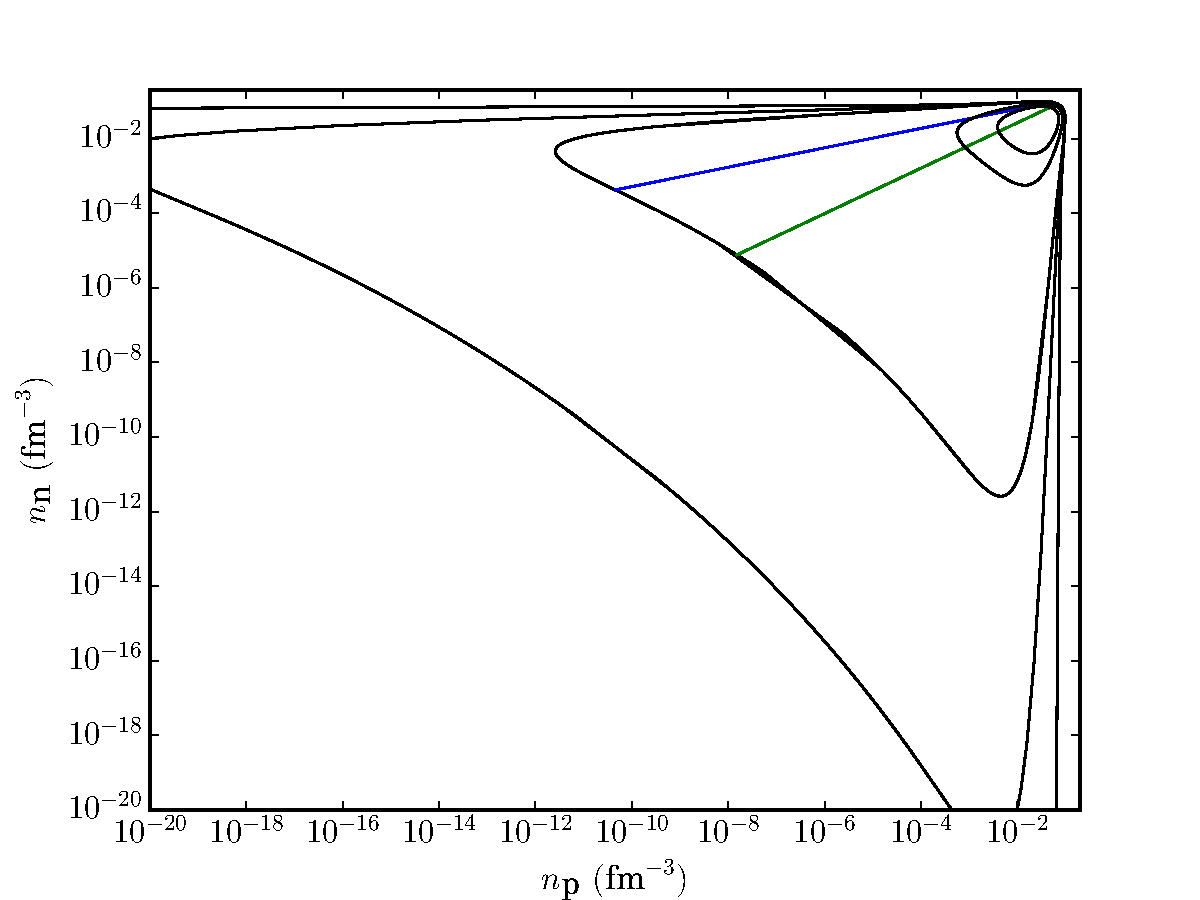
\includegraphics[width=0.9\textwidth]{PhaseBoundaryDensity.pdf}
\vspace*{-0.35cm}
\caption{ Phase boundaries for a variety of temperatures with LS Skyrme.}
\vspace*{-0.7cm}
\end{figure}

\end{document}
